\documentclass[12pt, letterpaper]{article}

\usepackage{spreamble}
\usepackage[bottom=2cm, top=2cm, left=1.5cm, right=1.5cm]{geometry}
\usepackage{graphicx}
\usepackage{multirow}

\title{\textbf{Practical 5} \\[1ex] \large Penetration Testing Report}
\author{Ian Zou}

\begin{document}

\maketitle

\clearpage
\section{Executive Summary}

On April 10th, 2026, Ian Zou (hereby referenced as \textit{The
Pentester}) was tasked with performing a black-box
penetration test on \textit{Fazbear Entertainment}'s internal
infrastructure as part of a security evaluation. \bigskip

As time was sensitive, the pentester was given the maximum of 3 hours to
find as many security vulnerabilities that were present on
\textit{Fazbear Entertainment}'s remote server. The pentester was able to
identify several security vulnerabilities in this period of time,
including many critical vulnerabilities that allowed for internal
database enumeration, unauthorized access to confidential
information, privilege escalation, and unauthorized logins.

\section{Engagement Overview}

\subsection{Goals}

The primary objective of this penetration test is to identify any and
all security vulnerabilities present in \textit{Fazbear
Entertainment}'s internal infrastructure. The security
vulnerabilities specifically targeted range from minor
misconfigurations of the frontend to critical vulnerabilities that
may expose sensitive information to unauthorized users. This report
will document all security vulnerabilities identified and any
remediating actions needed to be taken, and is to be delivered to
Michael Link, who will act as the middleman between the pentester and the
client (\textit{Fazbear Entertainment}).

\subsection{Scope}

The pentester was tasked with conducting a penetration test on the
\texttt{5.55.53.53}
remote server, which itself is a sandboxed replica of \textit{Fazbear
Entertainment}'s internal infrastructure. This remote server hosts two
applications: \textbf{Fazbear Parts \& Service} (port \texttt{8091}), and
\textbf{Fazbear Staff Portal} (port \texttt{8092}). \bigskip

As part of the penetration test, the pentester was assigned a
specialized pod on the
\texttt{5.55.53.0/24} network, with the IP address \texttt{5.55.53.3}.
Connection to this device was enabled via \textit{NoVNC} through the \textit{NDG
Portal}. All internal testing was restricted to this device. \bigskip

The pentester was given the explicit permission to tamper with and exploit these
services in whatever way the pentester sees fit for the purpose of identifying
potential security vulnerabilities, including but not limited to:

\begin{itemize}
  \item Network scanning,
  \item File injection,
  \item Command \& SQL injection,
  \item Cross-site scripting,
  \item Credential changing,
  \item etc.
\end{itemize}

Should the pentester conduct any irreversible changes that damage the
internal infrastructure being tested on or in any way make the remote
server behave in an unpredicted way, the pentester has been given the
ability to reset these changes to a fresh, untampered snapshot of the
server. No changes will be conducted to the live environment
currently served to the staff. All confidential information obtained
in the process of the penetration test should be documented with
redactions. Any files obtained from the remote server onto the attack
pod should be documented and promptly destroyed.

\section{Technical Report}

\subsection{Introduction}

This section contains a detailed, technical analysis and overview of
the security vulnerabilities that were found over the course of the
penetration test. Each section will contain the severity of the
vulnerability, reproducible steps to recreate an instance of the
vulnerability, possible risks and compromised information, and
remediation steps and action to be taken by a system administrator. \bigskip

Each security vulnerability's severity will be assessed using the
industry standard Common Vulnerability Scoring System \textit{(CVSS
v.3.1)} as a baseline, with modifications tailored against its
relevance to the client, \textit{Fazbear Entertainment}. A
qualitative risk rating will be given based on this scale:

\bigskip
\begin{table}[!ht]
  \centering
  \resizebox{0.4 \textwidth}{!}{
    \begin{tabular}{|l|l|}
      \hline
      \cellcolor{RoyalPurple}{\color[HTML]{FFFFFF} \textbf{Critical}}      &
      {\color{RoyalPurple} 9.0 - 10.0} \\ \hline
      \cellcolor{red}{\color[HTML]{FFFFFF} \textbf{High}}          &
      {\color{red} 7.0 - 8.9}  \\ \hline
      \cellcolor{orange}{\color[HTML]{FFFFFF} \textbf{Medium}}        &
      {\color{orange} 4.0 - 6.9}  \\ \hline
      \cellcolor{green}{\color[HTML]{FFFFFF} \textbf{Low}}           &
      {\color{green} 1.0 - 3.9}  \\ \hline
      \cellcolor{cyan}{\color[HTML]{FFFFFF} \textbf{Informational}} &
      {\color{cyan} 0.0 - 0.9}  \\ \hline
    \end{tabular}%
  }
  \caption{Qualitative risk rating scale.}
  \label{cvss}
\end{table}
\FloatBarrier
\bigskip

Two other factors have also been considered in evaluating the adjusted CVSS
score tailored to how impactful or devastating a particular security
vulnerability is for \textit{Fazbear Entertainment}:

\bigskip
\begin{table}[!ht]
  \centering
  \resizebox{0.4 \textwidth}{!}{
    \begin{tabular}{|l|l|}
      \hline
      \cellcolor[HTML]{000080}{\color[HTML]{FFFFFF}
      \textbf{Likelihood}} &
      \cellcolor[HTML]{000080}{\color[HTML]{FFFFFF} \textbf{Impact}} \\ \hline
      \textcolor{RoyalPurple}{Very High} &
      \textcolor{RoyalPurple}{Catastrophic} \\ \hline
      \textcolor{red}{High} &
      \textcolor{red}{Serious} \\ \hline
      \textcolor{orange}{Moderate} &
      \textcolor{orange}{Moderate} \\ \hline
      \textcolor{green}{Low} &
      \textcolor{green}{Tolerable} \\ \hline
      \textcolor{cyan}{Insignificant} &
      \textcolor{cyan}{Insignificant} \\ \hline

    \end{tabular}%
  }
  \caption{Additional factors that determine adjusted CVSS score.}
  \label{other-factors}
\end{table}
\FloatBarrier
\bigskip

\clearpage
\section*{C1 - SQL Injection: Admin Password Bypass}

\begin{table}[!ht]
  \centering
  \renewcommand{\arraystretch}{1.8} % Increases row height for a cleaner look
  \begin{tabular}{|c|c|c|c|c|}
    \hline
    \multirow{3}{*}{\textcolor{RoyalPurple}{\textbf{\huge 9.6}}} &
    \multicolumn{4}{c|}{\textbf{Adjusted CVSS v3.1 Score}} \\ \cline{2-5}
    & \textbf{Vector} &
    \multicolumn{3}{c|}{AV:N/AC:L/PR:N/UI:N/S:C/C:H/I:H/A:L} \\ \cline{2-5}
    & \textbf{Likelihood} & \textcolor{RoyalPurple}{\textbf{Very High}}
    & \textbf{Impact} & \textcolor{red}{\textbf{Serious}} \\ \hline
    \multicolumn{5}{|c|}{\textbf{Affected Systems}} \\ \hline
    \textbf{IP Address} & \textbf{Port} &
    \multicolumn{2}{c|}{\textbf{Service}} & \textbf{Version} \\ \hline
    \texttt{5.55.53.53} & \texttt{8091} & \multicolumn{2}{c|}{Apache}
    & \texttt{2.4.66} \\ \hline
  \end{tabular}
\end{table}
\FloatBarrier

\subsection*{Details}

Unsanitized form on the \texttt{/login.php} endpoint allows for an SQL
injection and thus a simple SQL password bypass, granting any
unprivileged user access to the \texttt{admin} account.

\subsection*{Confirmation}

Access the login page at \texttt{http://5.55.53.53:8091/login.php},
and attempt to login with the following payload which bypasses the
password field for the \texttt{admin} account:

\begin{figure}[!ht]
  \centering
  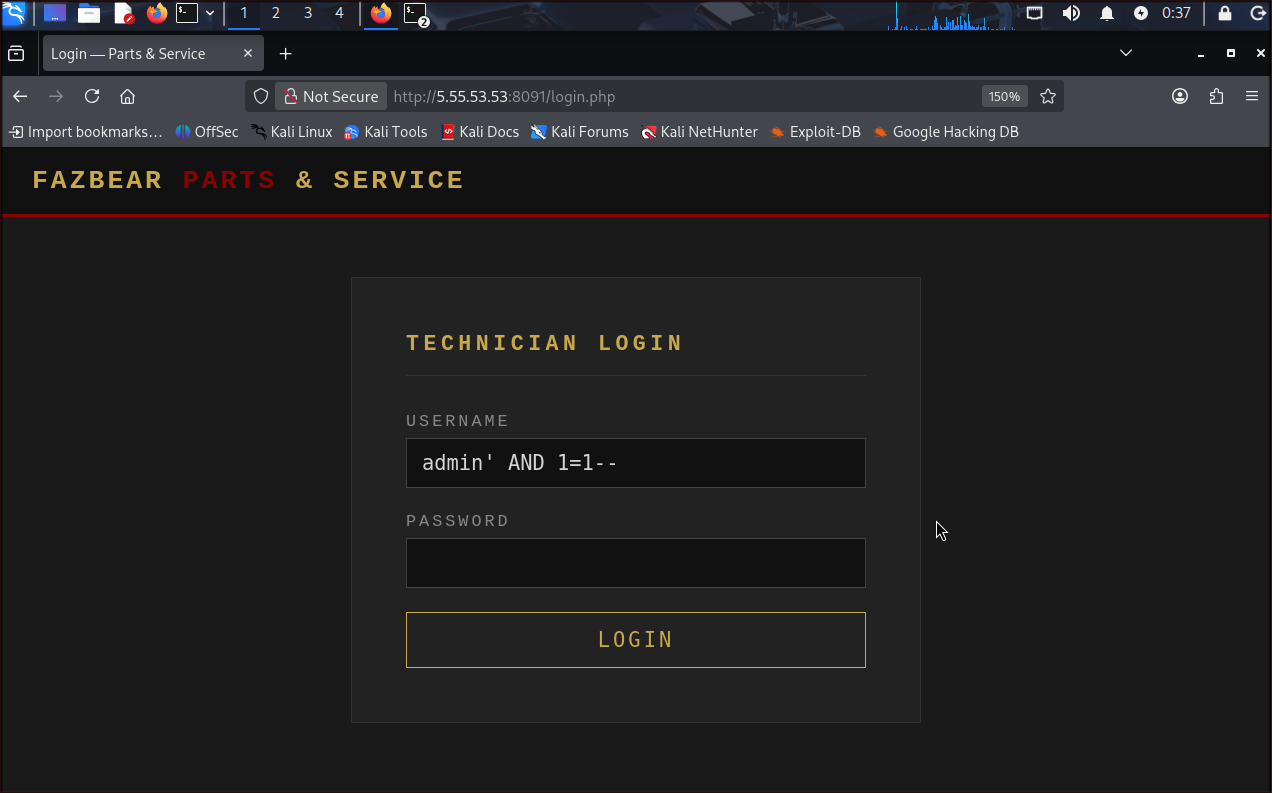
\includegraphics[width=0.9\textwidth]{./l2-01.png}
\end{figure}
\medskip

The login should succeed, and authentication will be granted to the
unprivileged user.

\begin{figure}[!ht]
  \centering
  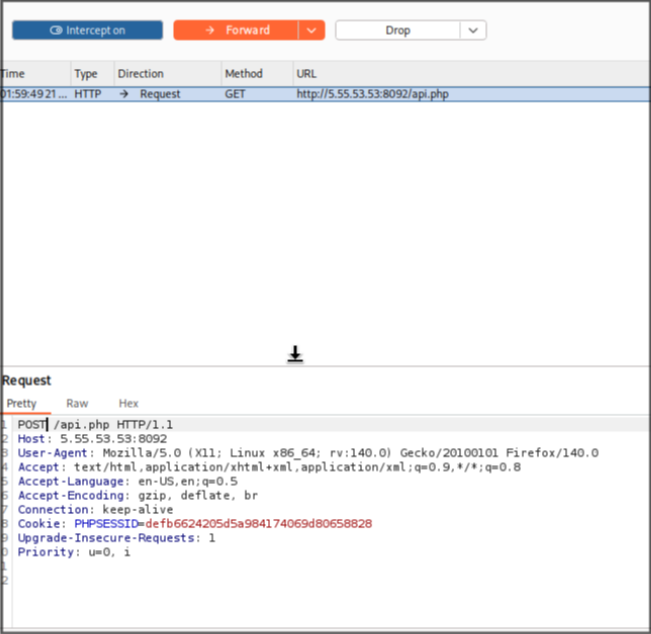
\includegraphics[width=0.9\textwidth]{./l2-02.png}
\end{figure}
\medskip

\subsection*{Impact}

Gaining access to an \texttt{admin} account as an unprivileged user
is an extremely critical security vulnerability, and will surely
compromise the entire infrastructure. An \texttt{admin} account can
perform almost virtually task on the remote server, such as uploading
malicious files, enumerating internal databases, changing passwords,
or leaking confidential information.

\subsection*{Remediation}

In order to prevent an SQL injection from occurring, sanitized input
forms and parameterized queries should be used. Sanitizing inputs
prevents certain escape characters from being used to break out of
SQL query parameters and providing malicious SQL keywords.
Parameterized queries, on the other hand, prevent SQL injections
altogether by decoupling the input from being concatenated directly
into the SQL query itself.

\clearpage
\section*{C2 - SQL Injection: UNION SELECT \& Database Enumeration}

\begin{table}[!ht]
  \centering
  \renewcommand{\arraystretch}{1.8} % Increases row height for a cleaner look
  \begin{tabular}{|c|c|c|c|c|}
    \hline
    \multirow{3}{*}{\textcolor{RoyalPurple}{\textbf{\huge 9.8}}} &
    \multicolumn{4}{c|}{\textbf{Adjusted CVSS v3.1 Score}} \\ \cline{2-5}
    & \textbf{Vector} &
    \multicolumn{3}{c|}{AV:N/AC:L/PR:N/UI:N/S:C/C:H/I:H/A:N} \\ \cline{2-5}
    & \textbf{Likelihood} & \textcolor{RoyalPurple}{\textbf{Very High}}
    & \textbf{Impact} & \textcolor{RoyalPurple}{\textbf{Catastrophic}} \\ \hline
    \multicolumn{5}{|c|}{\textbf{Affected Systems}} \\ \hline
    \textbf{IP Address} & \textbf{Port} &
    \multicolumn{2}{c|}{\textbf{Service}} & \textbf{Version} \\ \hline
    \texttt{5.55.53.53} & \texttt{8091} & \multicolumn{2}{c|}{Apache}
    & \texttt{2.4.66} \\ \hline
  \end{tabular}
\end{table}
\FloatBarrier

\subsection*{Details}

The \texttt{/parts.php} endpoint has a vulnerable search bar, of
which the query is susceptible to a \texttt{UNION SELECT} SQL
injection. Since the \texttt{/parts.php} endpoint is accessible
without authentication, this security vulnerability essentially
allows for any unprivileged user to enumerate the underlying
\textit{SQLite} database.

\subsection*{Confirmation} % TODO

\subsection*{Impact}

The ability to enumerate the entirety of the internal \textit{SQLite}
database is catastrophic: it grants any user the ability to dump the
accounts and corresponding credentials of every registered user in
the system, every single order made by every single user, every
single part that that exists in the database, and even some
confidential or staff-only items that should be accessible to any
unprivileged user.

\subsection*{Remediation}

In order to prevent an SQL injection from occurring, sanitized input
forms and parameterized queries should be used. Sanitizing inputs
prevents certain escape characters from being used to break out of
SQL query parameters and providing malicious SQL keywords.
Parameterized queries, on the other hand, prevent SQL injections
altogether by decoupling the input from being concatenated directly
into the SQL query itself.

\clearpage
\section*{H1 - File Inclusion \& Path Traversal}

\begin{table}[!ht]
  \centering
  \renewcommand{\arraystretch}{1.8} % Increases row height for a cleaner look
  \begin{tabular}{|c|c|c|c|c|}
    \hline
    \multirow{3}{*}{\textcolor{red}{\textbf{\huge 7.8}}} &
    \multicolumn{4}{c|}{\textbf{Adjusted CVSS v3.1 Score}} \\ \cline{2-5}
    & \textbf{Vector} &
    \multicolumn{3}{c|}{AV:N/AC:L/PR:N/UI:N/S:C/C:H/I:H/A:N} \\ \cline{2-5}
    & \textbf{Likelihood} & \textcolor{red}{\textbf{High}}
    & \textbf{Impact} & \textcolor{orange}{\textbf{Moderate}} \\ \hline
    \multicolumn{5}{|c|}{\textbf{Affected Systems}} \\ \hline
    \textbf{IP Address} & \textbf{Port} &
    \multicolumn{2}{c|}{\textbf{Service}} & \textbf{Version} \\ \hline
    \texttt{5.55.53.53} & \texttt{8091} & \multicolumn{2}{c|}{Apache}
    & \texttt{2.4.66} \\ \hline
  \end{tabular}
\end{table}
\FloatBarrier

\subsection*{Details}

A document viewer located at the \texttt{/docs.php} endpoint is
vulnerable to a path traversal and file inclusion attack. It can be
used to read a file off of the remote server's internal filesystem,
or used as an setup for a much more catastrophic attack.

\subsection*{Confirmation}

Recognize that the content of the documentation is taken directly
from a file within some internal server directory, as specified by
the \texttt{?page} parameter in the URL.

\begin{figure}[!ht]
  \centering
  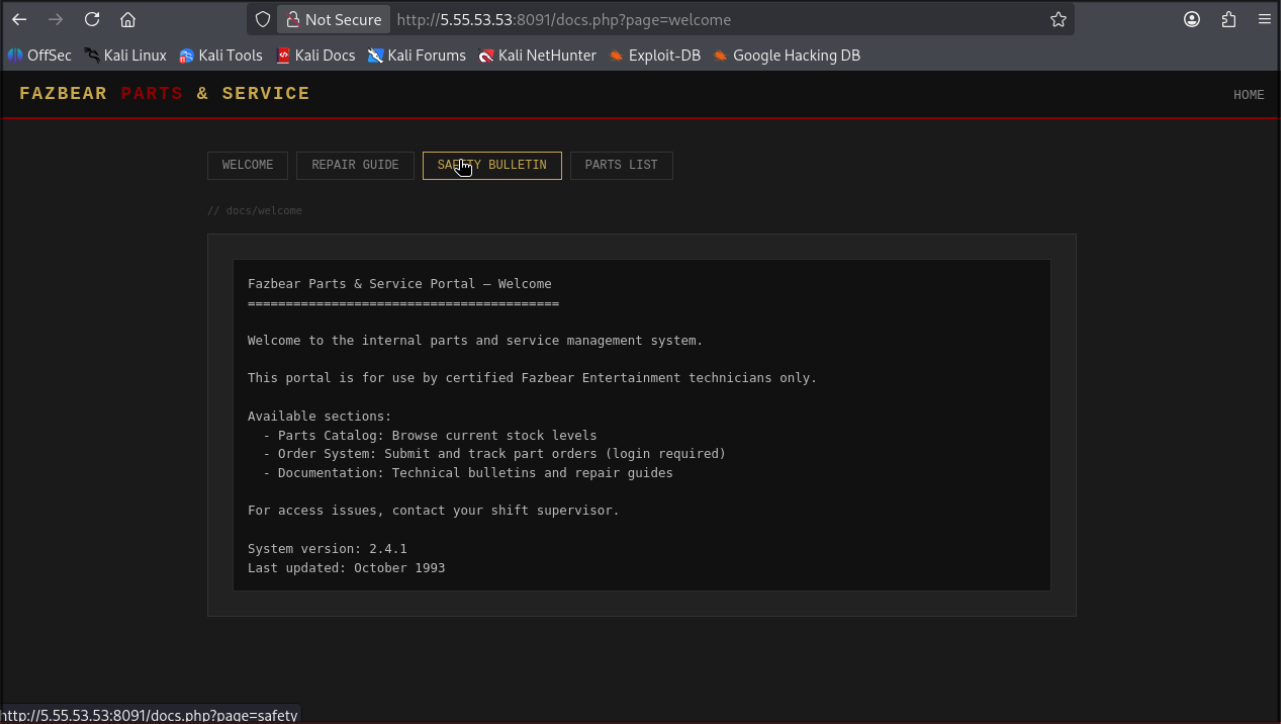
\includegraphics[width=0.9\textwidth]{./h1-01.png}
\end{figure}

We can edit the \texttt{?page} and attempt to point to some invalid
file. If we set \texttt{?page=../}, we can observe it attempt to
strip away the relative path but inadvertently show us the underlying PHP error.

\begin{figure}[!ht]
  \centering
  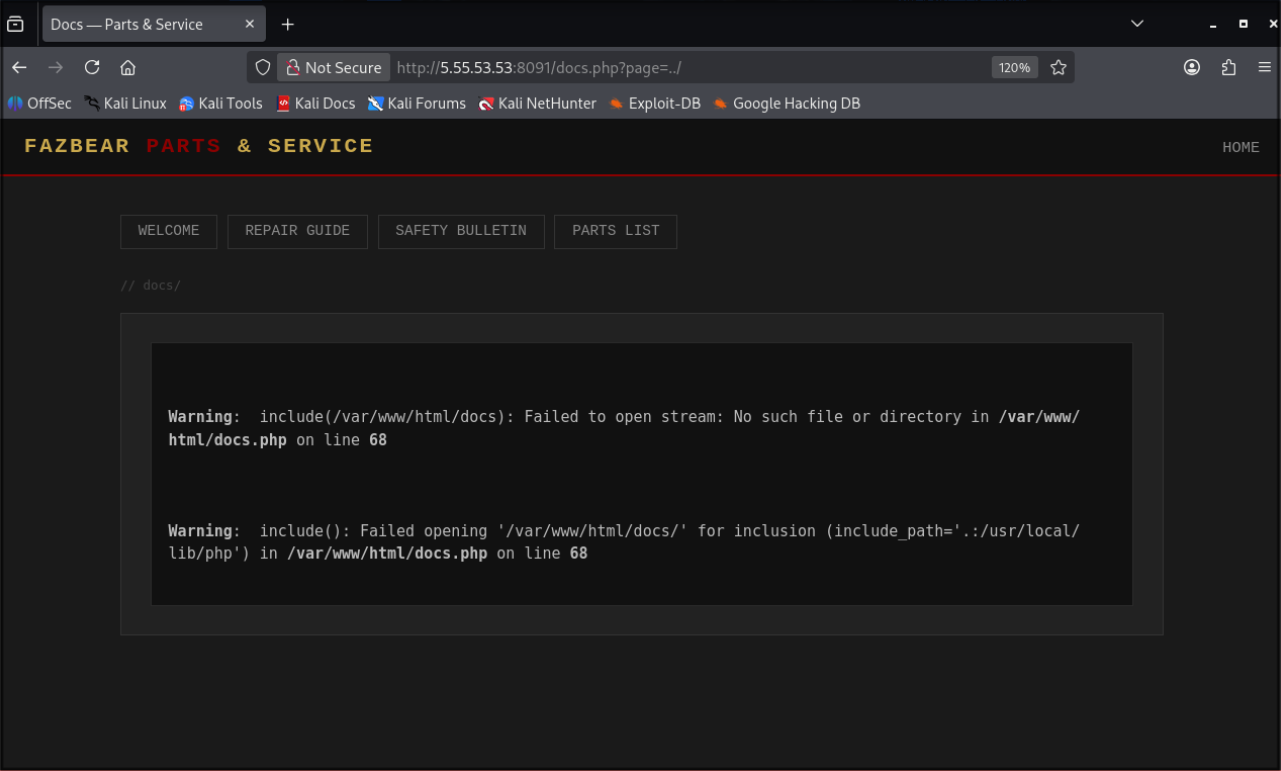
\includegraphics[width=0.9\textwidth]{./h1-02.png}
\end{figure}

The presence of \texttt{include()} and the fact that \texttt{?page}
is being fed directly into this function as a parameter was ample
evidence to indicate a file traversal vulnerability. After some
testing, we concluded that the server cannot fully strip
\texttt{....//}, allowing for full path traversal. This is confirmed
by the following output indicating that PHP is now searching for a
nonexistent file in a parent directory:

\begin{figure}[!ht]
  \centering
  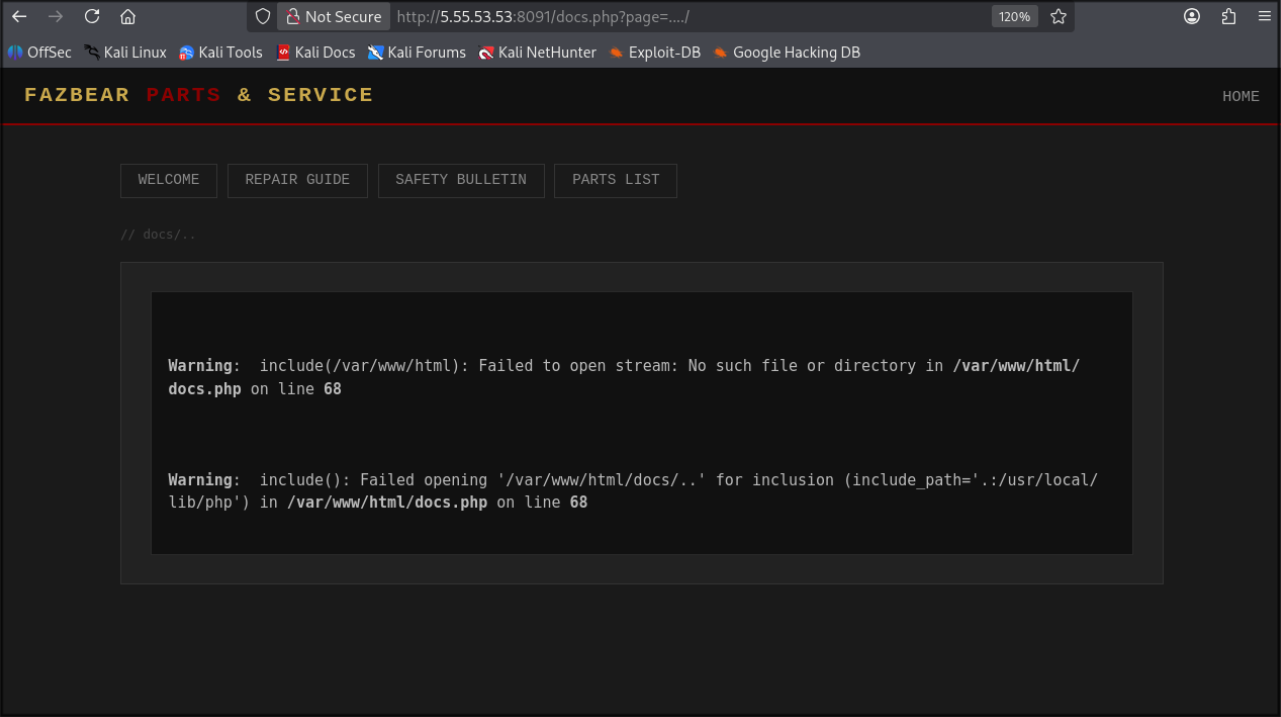
\includegraphics[width=0.9\textwidth]{./h1-03.png}
\end{figure}

This path traversal method was used to compromise sensitive
information stored in the home folder of the remote server's computer:

\begin{figure}[!ht]
  \centering
  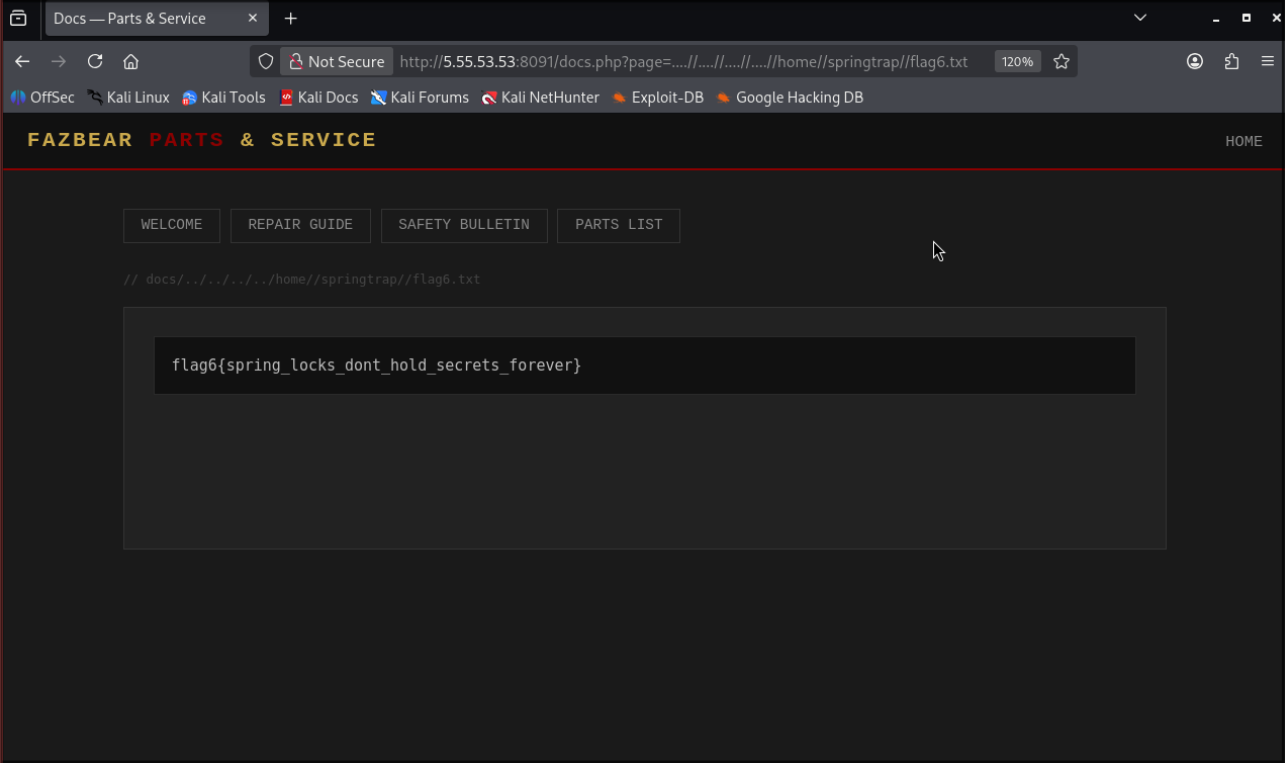
\includegraphics[width=0.9\textwidth]{./h1-04.png}
\end{figure}

\subsection*{Impact}

File traversal has the technical ability to enumerate the entire
filesystem of the remote server. The pentester was able to find
sensitive information given enough intelligence gathered from various
other attack vectors. The biggest impact is the ability for the file
traversal to include an uploaded file in a known directory. An
uploaded file may contain a malicious payload that can be exploited
in conjunction with this security vulnerability to establish a
devastating attack.

\subsection*{Remediation}

Use a whitelist of allowed files to be accessed by the code and
sanitize paths by removing \texttt{../} or patterns of the like. Do
not feed user input as a parameter directly into \texttt{include()}.

\clearpage
\section*{L1 - Unused Endpoint}

\begin{table}[!ht]
  \centering
  \renewcommand{\arraystretch}{1.8} % Increases row height for a cleaner look
  \begin{tabular}{|c|c|c|c|c|}
    \hline
    \multirow{3}{*}{\textcolor{orange}{\textbf{\huge 5.8}}} &
    \multicolumn{4}{c|}{\textbf{Adjusted CVSS v3.1 Score}} \\ \cline{2-5}
    & \textbf{Vector} &
    \multicolumn{3}{c|}{AV:N/AC:L/PR:N/UI:N/S:U/C:L/I:N/A:N} \\ \cline{2-5}
    & \textbf{Likelihood} & \textcolor{red}{\textbf{High}}
    & \textbf{Impact} & \textcolor{orange}{\textbf{Moderate}} \\ \hline
    \multicolumn{5}{|c|}{\textbf{Affected Systems}} \\ \hline
    \textbf{IP Address} & \textbf{Port} &
    \multicolumn{2}{c|}{\textbf{Service}} & \textbf{Version} \\ \hline
    \texttt{5.55.53.53} & \texttt{8091} & \multicolumn{2}{c|}{Apache}
    & \texttt{2.4.66} \\ \hline
  \end{tabular}
\end{table}
\FloatBarrier

\subsection*{Details}

Although not accessible by any normal means, the \texttt{/archive}
endpoint has still been left open and accessible should the URL be
manually inputted.

\subsection*{Confirmation}

Using Gobuster, a tool for fuzzing and finding exposed endpoints on a
given webserver given a wordlist, we were very easily able to
find this endpoint with a common lowercase wordlist from Dirbuster:

\begin{minted}[
        framesep=2mm,
        baselinestretch=1.2,
        breaklines,
    ]{bash}
    gobuster dir -u http://5.55.53.53:8091 -w /usr/share/wordlists/dirbuster/directory-list-lowercase-2.3-small.txt
\end{minted}

\begin{figure}[!ht]
  \centering
  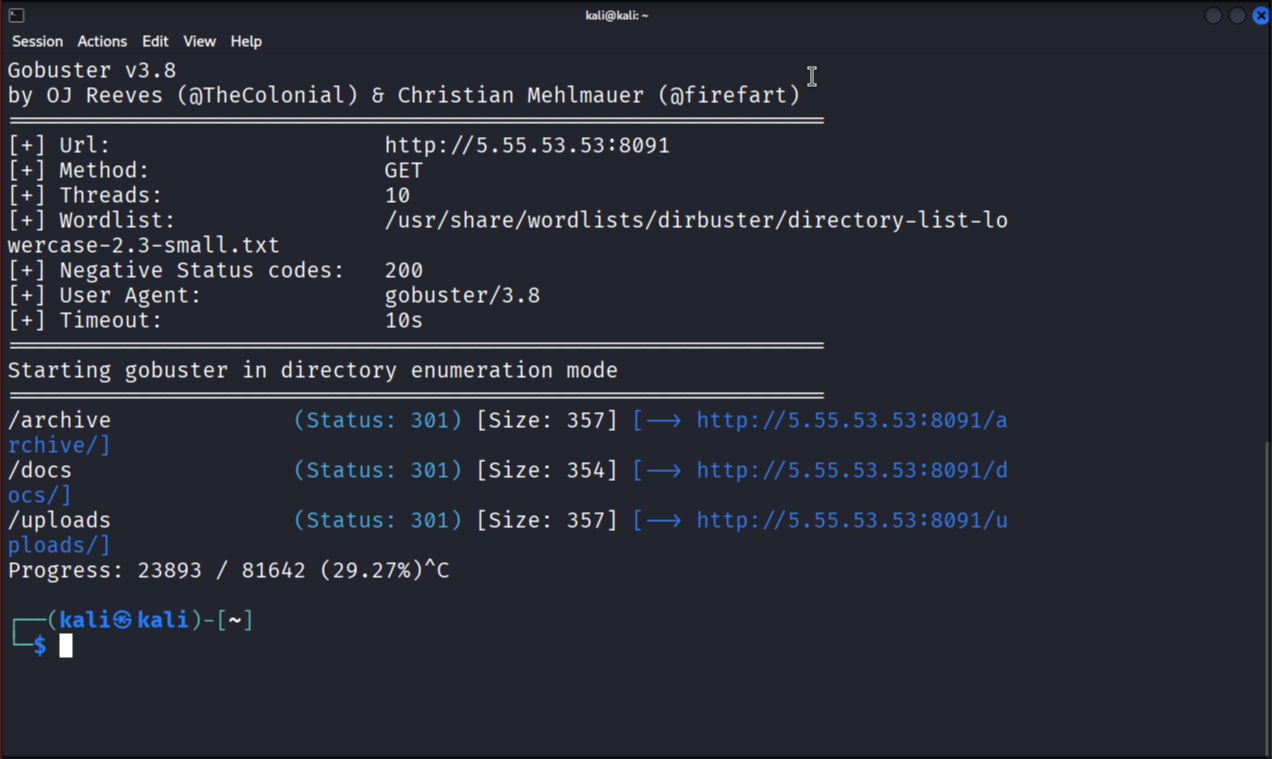
\includegraphics[width=0.9 \textwidth]{./l1-01.png}
\end{figure}
\medskip

Furthermore, no authentication was required to access this endpoint,
which allowed for the download and access of an internal log
\texttt{parts.txt}, containing sensitive information.

\begin{figure}[!ht]
  \centering
  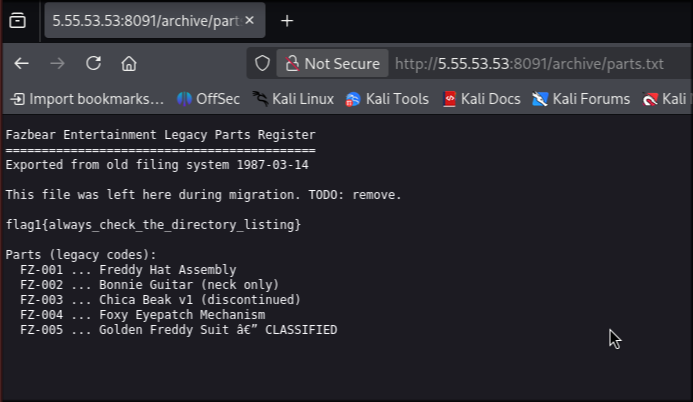
\includegraphics[width = 0.9\textwidth]{./l1-02.png}
\end{figure}
\bigskip

\subsection*{Impact}

Should this \texttt{/archive} endpoint have been an active endpoint
used to archive confidential information, this simple
misconfiguration could have been devastating. Hidden (but accessible)
endpoints are common misconfigurations, but their risk vary
significantly depending on the type of information that is hosted. In
this case, old archives could contain sensitive information about
\textit{Fazbear Entertainment}'s internal business or reveal
information to attackers regarding other vulnerable parts of the
server infrastructure.

\subsection*{Remediation}

Web pages that are hosted by a web server will be accessible as long
as their exact URL is known. Therefore, it is not a good idea to have
the only barrier of entry to some arbitrary endpoint containing
sensitive information be a hidden URL, as it is possible to use
automated fuzzing tools to enumerate and uncover such web pages.
\bigskip

It is a good idea to always enforce authentication to endpoints which
contain sensitive information, or otherwise take down old endpoints
that are not meant to be accessible anymore.

\end{document}
